\section{Our Improvements}\label{sec:improvements}

In this chapter, we introduce some modifications or additions to the solution proposed by Peng et al. in \cite{peng_main_paper}, aiming to improve the robot's behavior in more general and complex environments.

\subsection{Subgoals and RRT*}
\todo[inline]{TO IMPROVE}
As described in Section \ref{sec:mpc}, the solution provided by the MPC is the input that minimizes the cost function while satisfying all the constraints. When an obstacle lies between the start and the goal positions (as illustrated in Figure \todo{Add Figure num}), the robot must get around it in order to approach the goal. However, it would require the robot to deliberately increase its distance from the goal before reducing it. It implies that the MPC should return a sub-optimal solution, though one that minimizes the cost function could exist. Consequently, the previous approach cannot guarantee goal attainment in such cases.\\
To address this, we compute a path from the start to the goal position using RRT*. Then, we request the humanoid to reach sequentially all the \textit{subgoals}, namely the nodes of the tree in the path from the start to the goal. In this way, we ensure that the MPC produces feasible control inputs while adhering to the original cost-minimization framework, and the humanoid can successfully reach the goal.\\
The RRT* algorithm is used to compute fast a collision-free path, while minimizing the cost of the path, i.e. the sum of the edges' cost connecting the start to the goal node. Whenever a new node $j$ is added to the tree, the cost of the each $e_{i,j}$ connecting it to node $i$ is defined as:
$$ cost(e_{i, j}) \coloneqq  cost(path_{i,start})\, +\,dist(i, j) + e^{-clearance(j)}. $$
It is the sum of the cost of the path from $j$'s parent to the initial node, the Euclidean distance from the position represented by $i$ to the one represented by $j$, and the exponential of the negative clearance (namely, the distance of $j$ from the closest obstacle) of the new node.

FIGURE CAPTION:
In this Figure, in order to reach the goal, the robot must first overcome the obstacle by reaching the red star. Indeed, the RRT* solution contains 3 nodes: the start, the star, and the goal positions. The first goal provided to the robot is the star, which represents a subgoal. Once it has been reached with the standard framework, the original goal is provided to the MPC. With this approach it is possible for the humanoid to travel along a path that would be unfeasible by just using the MPC.



\subsection{Unknown Environments}
\begin{figure}[h]
    \centering
    % First row
    \begin{subfigure}{0.20\textwidth}
        \centering
        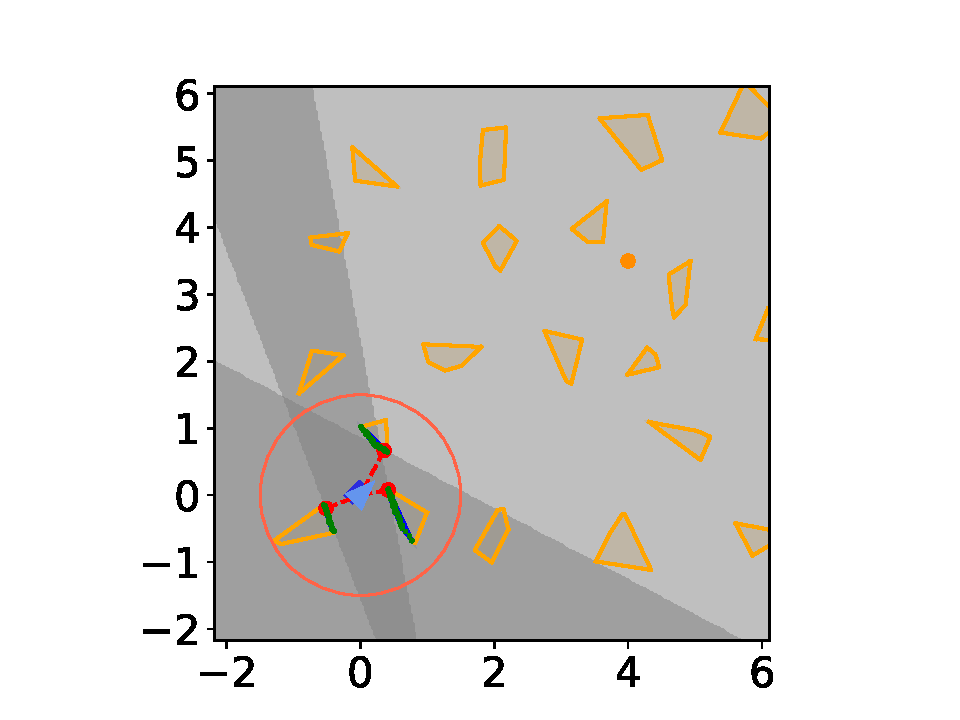
\includegraphics[width=\textwidth]{../figures/Simulations/sim2unkenv/frame_0.pdf}
    \end{subfigure}%
    \hfill
    \begin{subfigure}{0.20\textwidth}
        \centering
        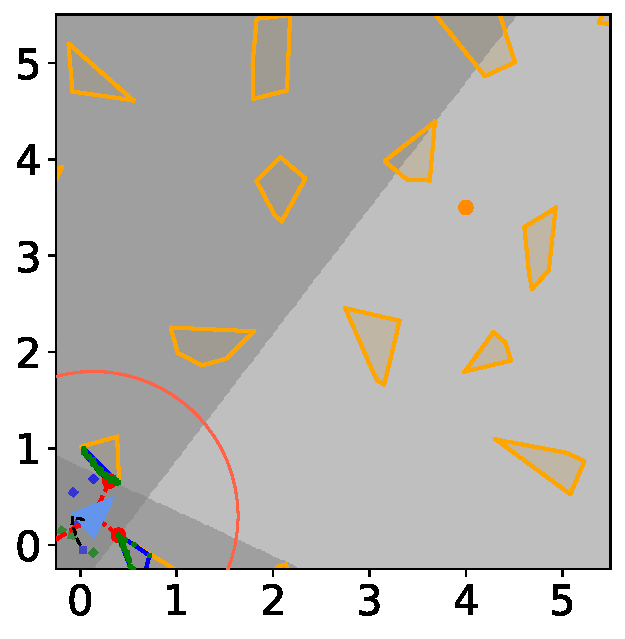
\includegraphics[width=\textwidth]{../figures/Simulations/sim2unkenv/frame_1.pdf}
    \end{subfigure}%
    \hfill
    \begin{subfigure}{0.20\textwidth}
        \centering
        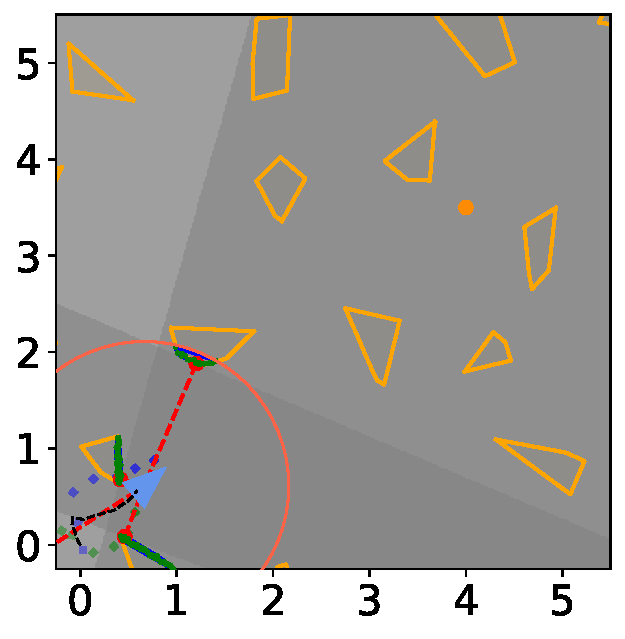
\includegraphics[width=\textwidth]{../figures/Simulations/sim2unkenv/frame_2.pdf}
    \end{subfigure}%
    \hfill
    \begin{subfigure}{0.20\textwidth}
        \centering
        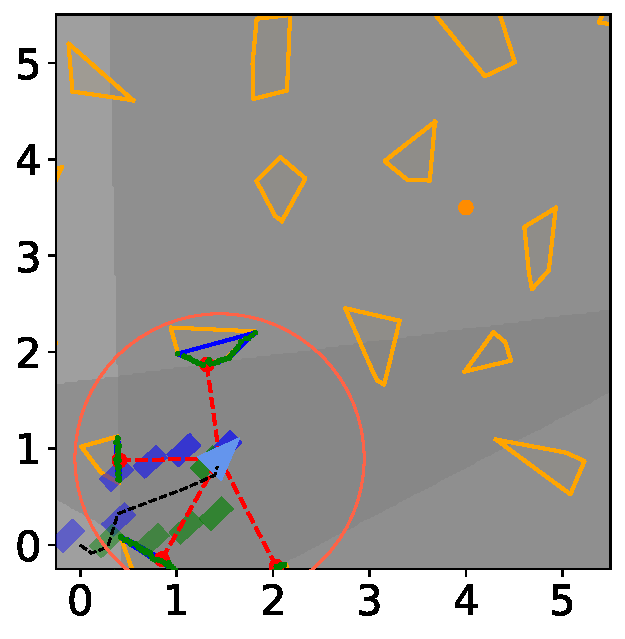
\includegraphics[width=\textwidth]{../figures/Simulations/sim2unkenv/frame_3.pdf}
    \end{subfigure}%
    \hfill
    \begin{subfigure}{0.20\textwidth}
        \centering
        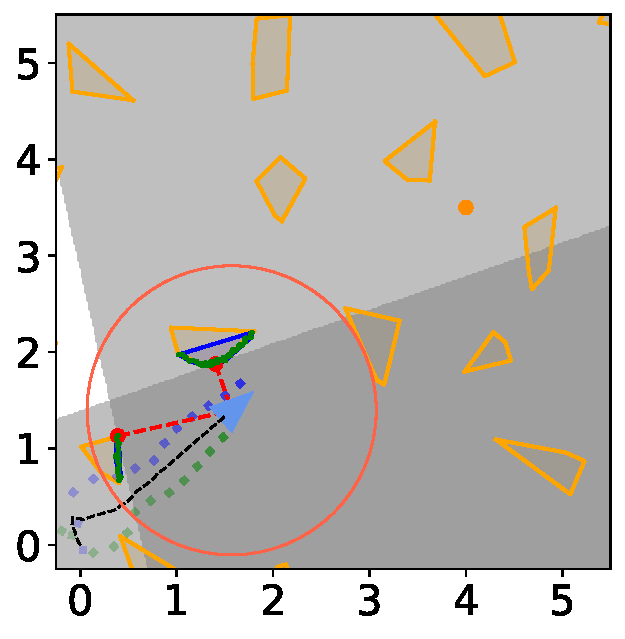
\includegraphics[width=\textwidth]{../figures/Simulations/sim2unkenv/frame_4.pdf}
    \end{subfigure}

    % Second row
    \begin{subfigure}{0.20\textwidth}
        \centering
        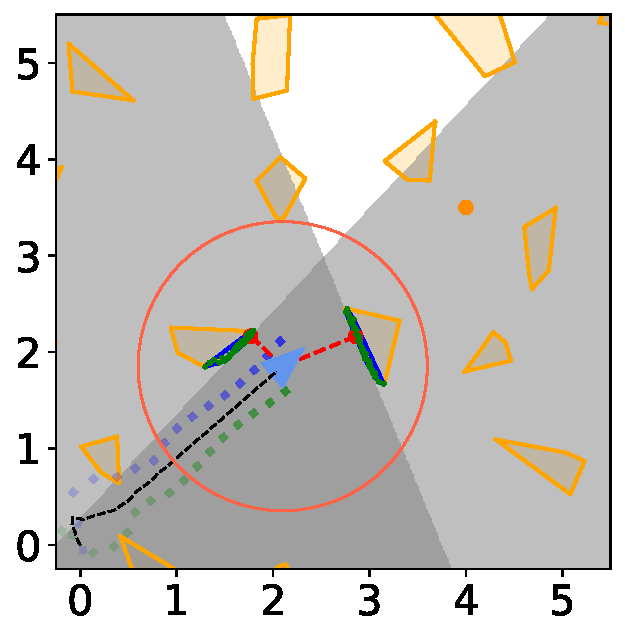
\includegraphics[width=\textwidth]{../figures/Simulations/sim2unkenv/frame_5.pdf}
    \end{subfigure}%
    \hfill
    \begin{subfigure}{0.20\textwidth}
        \centering
        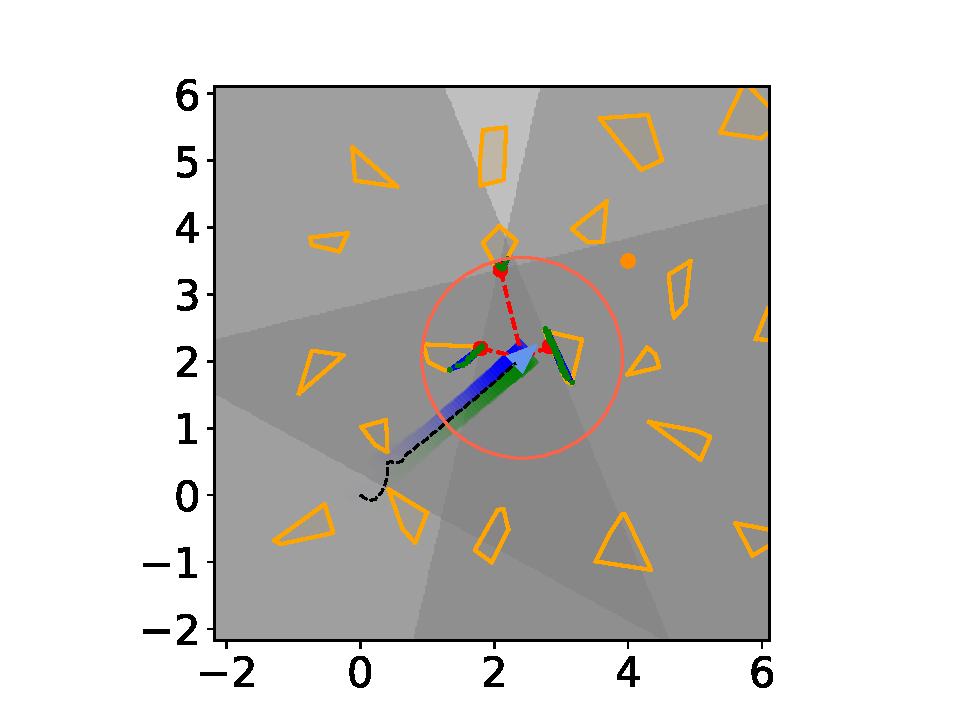
\includegraphics[width=\textwidth]{../figures/Simulations/sim2unkenv/frame_6.pdf}
    \end{subfigure}%
    \hfill
    \begin{subfigure}{0.20\textwidth}
        \centering
        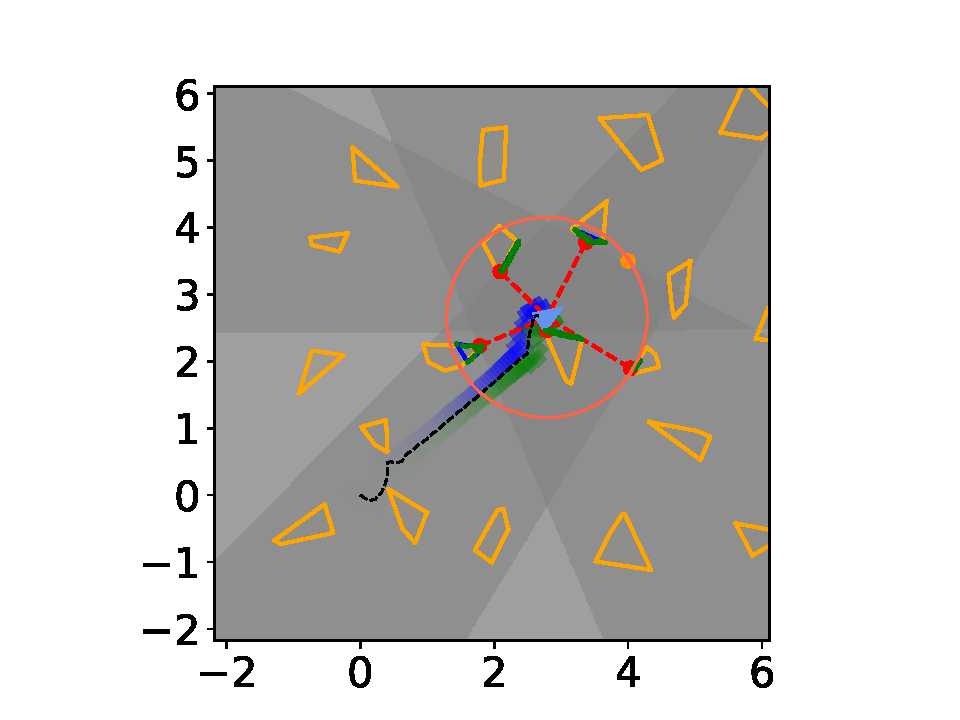
\includegraphics[width=\textwidth]{../figures/Simulations/sim2unkenv/frame_7.pdf}
    \end{subfigure}%
    \hfill
    \begin{subfigure}{0.20\textwidth}
        \centering
        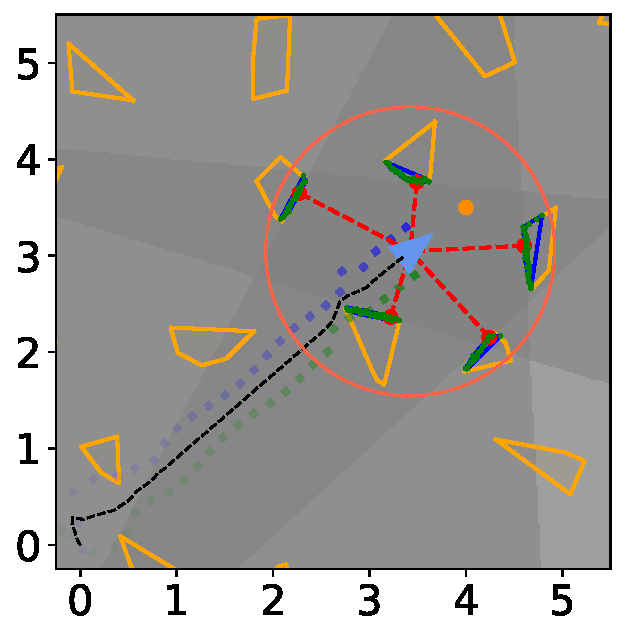
\includegraphics[width=\textwidth]{../figures/Simulations/sim2unkenv/frame_8.pdf}
    \end{subfigure}%
    \hfill
    \begin{subfigure}{0.20\textwidth}
        \centering
        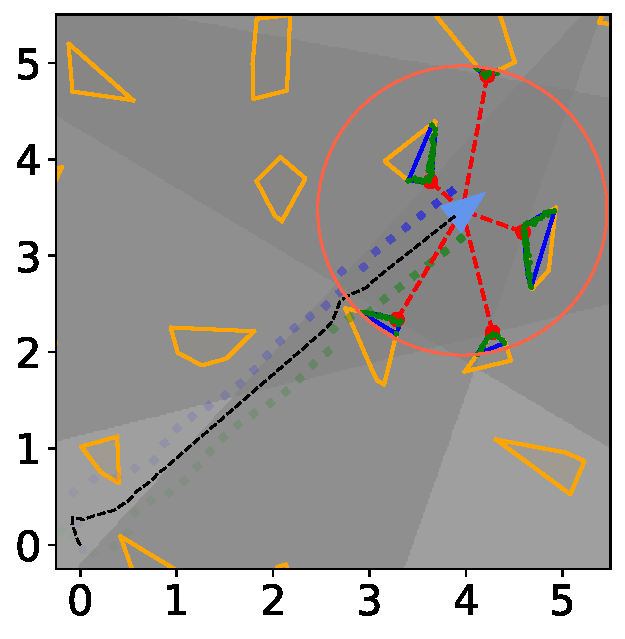
\includegraphics[width=\textwidth]{../figures/Simulations/sim2unkenv/frame_9.pdf}
    \end{subfigure}

    \caption[short]{This is a description.}
\end{figure}